% Chapter 1

\chapter{Background} % Main chapter title
\label{Chapter1} 
In order to understand the antenna design procedure as well as to interpret its performance outlined in the following chapters of this thesis, background knowledge on electromagnetics is essential. Therefore, background materials and mathematical concepts related to leaky-wave antennas and transformation electromagnetics are included in this chapter. In particular, this chapter presents a unified description of necessary concepts pertaining to antennas in general, different kinds of leaky-wave antennas and their design architecture, fixed-beam leaky-wave antennas in literature and extension of coordinate mapping to transformation electromagnetics. This chapter prepares the reader for Chapters \ref{Chapter2}, \ref{Chapter3} and \ref{Chapter4} in which the detailed design procedure and characterization of the proposed leaky-wave antenna is presented. 

%This chapter briefly presents Maxwell's equations and associated equations that describes wave propagation in dielectric media, leaky-wave antennas and their design architecture and mathematical concepts behind transformation electromagnetics and coordinate transformation. 
%%%%%%%%%%%%%%%%%%%%%%%%%%%%%%%%%%%%%%%%%%%%%%%%%%%%%%%%%%%%%%%%%%%%%%%%%%%%%%%%%%%%%%%%%%%%%%%%%%%
\section{Electromagnetics for antenna analysis}
Electric field intensity $\mathbf{E}$ is produced by electric charges. In contrast, magnetic field intensity $\mathbf{H}$ is caused by charges in motion. Time-varying electric and magnetic field intensities are coupled together and give rise to electromagnetic waves that propagates away from its source. This interaction of electric and magnetic field intensities was first realized by Scottish scientist James Clerk Maxwell. In 1861, Maxwell blended the individual works of Coulomb, Gauss, Faraday and appended his own intuition to demonstrate that time-varying electric and magnetic field intensities accompany each-other. Originally published in 1865 and later extended by Hertz, Heaviside, Lodge, and FitzGerald, Maxwell's equations describe the behavior of electromagnetic waves in a medium \cite{hunt2005}. Expressed in terms of electric and magnetic field intensities, the frequency-domain representation of these equations in the absence of sources are
%
\begin{subequations}
\begin{align}
\mathbf{\nabla} \cdot \mathbf{B}    &= 0 \label{eq:subeq1}\\ 
\mathbf{\nabla} \cdot \mathbf{D}    &= 0 \label{eq:subeq2}\\
\mathbf{\nabla} \times \mathbf{E} + j \omega \mu \mathbf{H} &= 0 \label{eq:subeq3}\\
\mathbf{\nabla} \times \mathbf{H} - j \omega \epsilon \mathbf{E} &= 0 \label{eq:subeq4}
\end{align} 
\end{subequations}
%
where $\epsilon$ and $\mu$ are the relative permittivity and permeability of the medium that supports the electromagnetic field, respectively. $\mathbf{D}$ and $\mathbf{B}$ are derived electric and magnetic flux densities. For a simple medium, Maxwell's equation can be extended into electromagnetic wave equations by taking the curl of the curl equations \ref{eq:subeq3} and \ref{eq:subeq4} and substituting the divergence equations \ref{eq:subeq1} and \ref{eq:subeq2} into the expression. The wave equations are expressed as
%
\begin{subequations}
\begin{align}
\mathbf{\nabla}^2 \mathbf{E} + \omega ^2 \epsilon \mu \mathbf{E}    &= 0 \label{eq:subeqb1} \\ 
\mathbf{\nabla}^2 \mathbf{H} + \omega ^2 \epsilon \mu \mathbf{H}    &= 0 
\end{align} 
\end{subequations}
%
The electromagnetic wave equations, also known as the Helmholtz equation, describes the propagation of electromagnetic wave through a transmission medium having a permittivity and permeability of $\epsilon$ and $\mu$, respectively. The solution of the wave Eq. \ref{eq:subeqb1} is the general plane wave 
%
\begin{equation} \label{eq:solution}
    \mathbf{E} = E_0 e^{\pm jkz + j\omega t}
\end{equation}
%
where $k$ is the wave number and is expressed as
\begin{equation}
 k = \dfrac{\omega}{\sqrt{\epsilon \mu}} 
 \end{equation}
% 
The impedance of the medium is represented by
%
\begin{equation} \label{eq:eta}
    \eta = \dfrac{E_0}{H_0} = \sqrt{\dfrac{\mu}{\epsilon}}
\end{equation}
%
The solution to Maxwell's equations in Eq. \ref{eq:solution} reveals that a bounded medium or a transmission line supports both forward and backward traveling wave. A forward traveling wave in a transmission line gives rise to reflected and transmitted waves when it encounters a segment of transmission line with mismatched impedance. \cite{sadiku2001}. The reflected wave or the backward traveling wave takes away a portion of the transmitted power intended to be transferred to the load. For the sake of maximum power transfer, a transmission line that feeds an antenna is generally expected to support forward wave only. 

%%%%%%%%%%%%%%%%%%%%%%%%%%%%%%%%%%%%%%%%%%%%%%%%%%%%%%%%%
\section{Antenna radiation parameters}

According to IEEE standards, antennas is defined as ``means for radiating and receiving radio waves" \cite{IEEE1983}. Antennas are employed in the first or last stage of a wireless system to couple guided electromagnetic waves from an electrical circuit into free-space and vice versa \cite{Stutzman2012, Balanis2005, Kraus2002}. Antennas come in various shapes and sizes depending on their applications. Design principles and radiation mechanisms differ widely for different categories of antennas.

In antenna engineering, the performance of an antenna is explained in terms of various antenna parameters. In order to interpret the results presented in this thesis, it is necessary for the reader to understand the significance of these widely used antenna parameters. Some common parameters are summarized below:
%
\begin{figure} [t]
\centering
\noindent
\begin{overpic}[scale=0.5]{Figures/Chapter0/Radiation/Antenna_lobes}
			\put(67,56){\footnotesize Main lobe}
			\put(-18,40){\footnotesize Back lobe}
			\put(-11,12){\footnotesize Null}
			\put(-7,-4){\footnotesize Side lobe}
			\put(30,2){\footnotesize $S_i$}
			\put(98,48){\footnotesize $S$}
			\put(68,-2){\footnotesize $D=\dfrac{S}{S_i}$}
	\end{overpic}
  
  \caption[Illustration of nulls, secondary lobes and directivity of an antenna radiation pattern.]{Illustration of nulls, secondary lobes and directivity of an antenna radiation pattern. The radiation pattern of the real antenna is shown by the solid line, while the dashed line represents an isotropic radiation. \cite{Stutzman2012}}
\label{fig:AntLobes}
\end{figure}

%
\begin{itemize}
\item \textit{Radiation pattern} is a plot of the strength of the emitted electromagnetic radiation in different directions. It describes the far-field behavior of an antenna. A sample radiation pattern of an antenna is presented in Fig. \ref{fig:AntLobes}.
\item  \textit{Half power beam width} describes the angle between the two directions where the radiation power of the main beam is half its maximum.
\item \textit{Main lobe} is the region with the highest radiated power density. Figure \ref{fig:AntLobes} presents different lobes of a radiation pattern from an antenna. Sidelobes are the largest of all undesired regions of the radiation pattern of the antenna. In contrast, backlobes are the lobes in the direction opposite to the main lobe. \textit{Sidelobe level} and \textit{Backlobe level} are the strengths of side lobe and backlobe radiation relative to the main lobe, respectively. Each lobes are separated by regions of zero field strength which are called \textit{nulls}.
\item  \textit{Directivity} provides a measure of how directive a radiation patten is. It is generally defined as the ratio of the radiation intensity in the direction of maximum radiation, to the radiation intensity averaged over all directions. In Fig. \ref{fig:AntLobes}, radiation intensities for an isotropic radiator and a given antenna are labeled as $S_i$ and $S$, respectively. Therefore, the directivity can be represented by $D=S / S_i$.
\item \textit{Bandwidth} of antenna is the range of frequencies over which the it demonstrates some given performance. In general, it is represented by the following equation:
%
\begin{equation}
  f(x)=\begin{cases}
    \dfrac{2(f_u - f_l)}{f_u + f_l} \times 100 \%, & \text{if bandwidth < 100\%}.\\
    \dfrac{f_u}{f_l}:1, & \text{if bandwidth > 100\%}.
  \end{cases}
\end{equation}
%
where $f_u$ and $f_l$ are the upper and lower cut-off frequencies \cite{chen2006}. Bandwidth of an antenna can be defined in terms of impedance, radiation pattern, and polarization. Impedance bandwidth represents the frequency range that allows satisfactory energy to be transferred from a transmission line to the antenna and vice versa. Pattern bandwidth is determined by specifying any of the antenna pattern parameters as either minimum or maximum according to the system requirements. Pattern bandwidth was primarily chosen to characterize the antenna presented in this thesis. 
\end{itemize}

The antenna parameters, such as the main beam direction, side and back lobe, beamwidth, etc, vary with frequency. Variations in the parameters result essentially from frequency-dependent distributions of electric and magnetic fields in the antenna structure. The antenna presented in this thesis has been designed upon specifying allowable sidelobe and backlobe levels for a broad bandwidth.

%%%%
%%%%%%%%%%%%%%%%%%%%%%%%%%%%%%%%%%%%%%%%%%%%%%%%%%%%%%%%%%%%%%%%%%%%%%%%%%%%%%%%%%%%%%%%%%%%%%%%%%%%%%%%%%%%%%%%%%%%%%%

\section{Leaky-wave antennas} \label{sec:LW}

%A leaky-wave antenna is defined as ``an antenna that couples power in small increments per unit length either continuously or discretely, from a traveling wave structure to free space.'' according to the IEEE Standard 145-1993, [cite: kai chang page 2294]. 
Leaky-wave antennas are a category of traveling-wave antennas. Traveling-wave antennas allow an electromagnetic wave to travel along a transmission line only in the forward direction and radiate energy in the process \cite{Balanis2005}\cite{ Walter1965}. The transmission line is long enough for the propagating wave so that it significantly decays before reaching the transmission line end. The structure often has a matched termination in order to prevent reflections. Either way, a negligible amount of power is left in the forward traveling wave at the terminating end of the traveling-wave structure. Traveling wave antennas can be divided into slow and fast wave antennas depending on the type of traveling-wave it uses for radiation mechanism. The fast wave traveling antennas are usually referred to as \textit{leaky-wave antennas} since the energy is continuously \textit{leaked} into free-space from the wave that propagates through the antenna structure \cite{Tamir1969}. Conversely, traveling-wave antennas that support slow waves are called \textit{slow-wave antennas}. Understanding the theoretical concept of fast and slow traveling-waves is necessary to analyze the radiation mechanism in a leaky-wave antenna. 
%%%%%%%%%%%%%%%%%%%%%%%%%%%%%%%%%%%%%%%%%%%%%%%%%%%%%%%

\subsection{Fast and slow-wave radiation} \label{fastslow}

\subsubsection{Slow-wave}
The terms fast or slow refers to the phase velocity of a traveling-wave mode as compared to the speed of light. Slow wave travels with a phase velocity slower than the speed of light ($v_p<c$) in that medium. Consequently, the propagation constant of a slow wave is greater than that of light and expressed as 
%
\begin{equation}
  \beta_{slow} = \dfrac{\omega}{v_p}  > k_0= \dfrac{\omega}{c} 
\end{equation}
%
%Propagating waves in most transmission lines are slow waves. Slow waves structures are used in microwave circuits to reduce velocity of the propagating wave.\cite{Milligan2005}. In the operation of high frequency (300 megahertz to 300 gigahertz) electron-tube devices, the electron beam must progress at the same velocity with the microwave signal \cite{Liao1985}. Phase velocity of an electromagnetic wave in standard waveguides is generally faster than that of light. On the other hand, since the electron beam travel only at velocities smaller than that of light. Therefore, it is impractical to accelerate the speed of an electron to such high velocity. A slow wave structure is incorporated in such cases so that the microwave signal can keep up with the electron beam of efficient interactions. 
Some example of slow wave structures are presented in Fig. \ref{fig:slowstrcture}. Helix type is the most widely used slow-wave structure since it is suitable for broadband (more than $>30\%$ bandwidth) applications. 

\begin{figure} [t!]
\centering
\noindent
\hspace*{\fill}
\subfloat[]{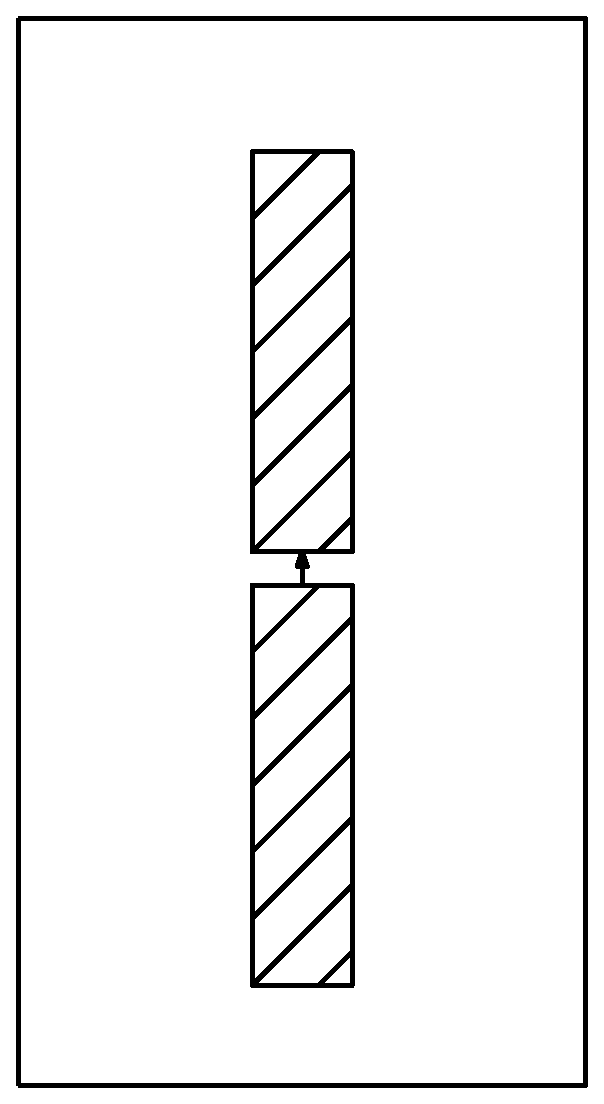
\includegraphics[scale=.5]{Figures/Chapter1/slow_waveguide_structure/a}} 
\hspace*{\fill}
\subfloat[]{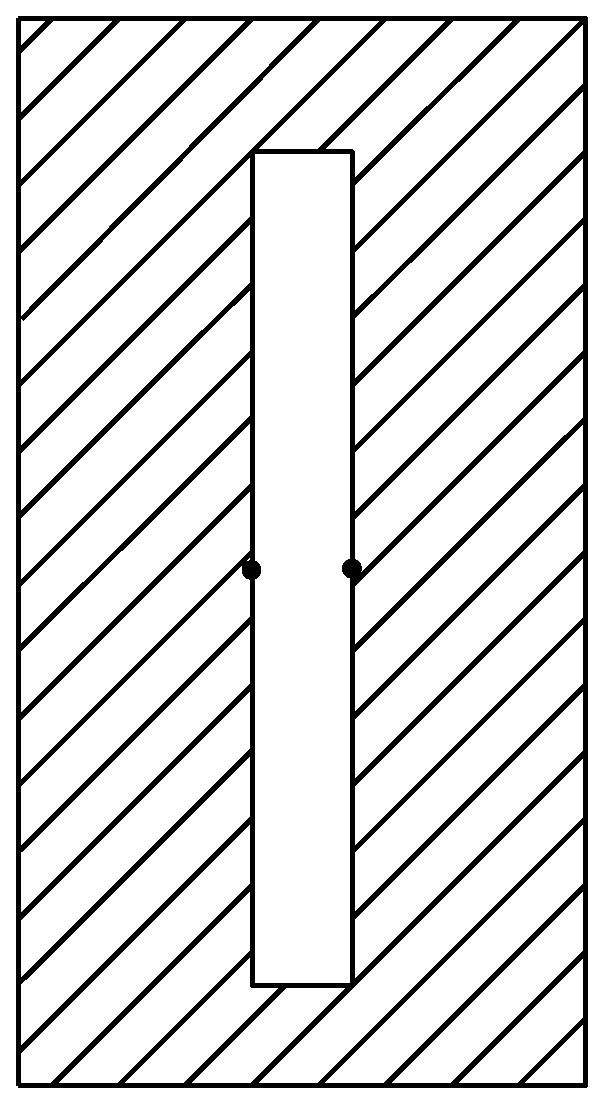
\includegraphics[scale=.5]{Figures/Chapter1/slow_waveguide_structure/b}} 
\hspace*{\fill}

\hspace*{\fill}
\subfloat[]{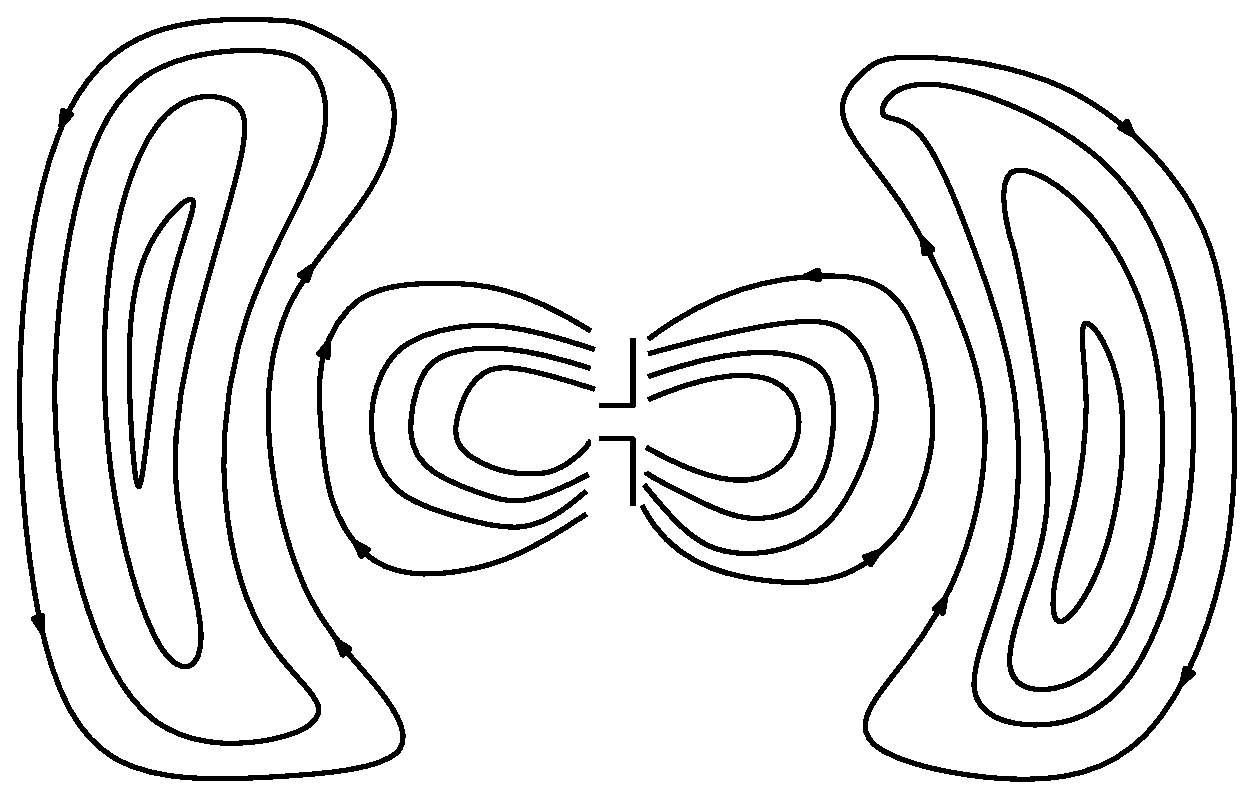
\includegraphics[scale=.5]{Figures/Chapter1/slow_waveguide_structure/c}}
\hspace*{\fill}
\subfloat[]{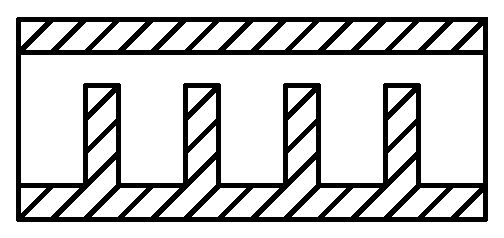
\includegraphics[scale=.5]{Figures/Chapter1/slow_waveguide_structure/d}} 
\hspace*{\fill}

\hspace*{\fill}
\subfloat[]{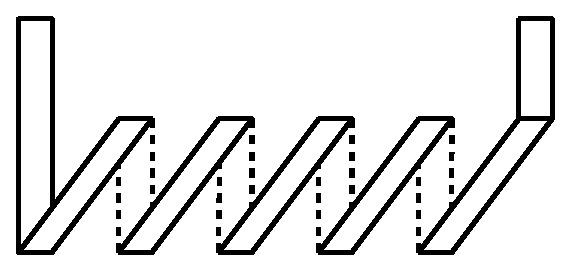
\includegraphics[scale=.5]{Figures/Chapter1/slow_waveguide_structure/e}} 
\hspace*{\fill}
  \caption[Models of simple slow-wave structures including folded-back transmission line, zigzag transmission line, interdigital transmission transmission line, corrugated transmission waveguide, and helix transmission line.]{Models of simple slow-wave structures. (a) Folded-back transmission line. (b) Zigzag transmission line. (c) Interdigital transmission transmission line. (d) Corrugated transmission waveguide. (e) Helix transmission line}
\label{fig:slowstrcture}
\end{figure}

The antenna proposed in the later chapters of this thesis is a leaky-wave antenna which utilizes fast waves as radiation mechanism. Therefore the following discussions are restricted to reviewing concepts of fast-wave radiation. 

%%%%%%%%%%%%%%%%%%%%%%%%%%%%%%%%%%%%%
\subsubsection{Fast-wave}
A fast wave has a phase velocity greater than the velocity of light in that medium ($v_p > \mathrm{c}$). Hence, the propagation constant of a fast wave is less than that of light as shown in the following equation
%
\begin{equation}
  \beta_{fast}= \dfrac{\omega}{v_p}  < k_0= \dfrac{\omega}{\mathrm{c}} 
\end{equation}
%
where $\omega $ is the operating frequency, $k_0$ and $\mathrm{c}$ is the wave constant and velocity of light in that medium, respectively. The fundamental $TE_{10}$ mode of a rectangular waveguide and higher order modes in a parallel plate waveguide are example of fast waves. A fast wave is capable of simultaneously \textit{leaking} energy into free-space \cite{Neto2010}\cite{felsen1994}.% Cherenkov radiation occurs when an electrically charged particle moves with higher phase velocity than the speed of light in the same medium . 

%
\begin{figure} [!t]
\centering
\noindent
\begin{overpic}[scale=0.8]{Figures/Chapter1/LWA_waveguide/LWA_waveguide}
		\put(51,40){\footnotesize $z$}
		\put(40,36){\footnotesize $y$}
		\put(97,19){\footnotesize $x$}
		\put(65,34){\footnotesize $\theta$}
		\put(94,28){\footnotesize Decay of}
		\put(94,25){\footnotesize LW mode}
		\put(-5,14){\footnotesize $\mathbf{E} = \hat{\mathbf{y}}e^{ - j \beta x}$}
    \put(70,37){\footnotesize $ \mathbf{E}(x,z) = \hat{\mathbf{y}}e^{ - j \beta x}e^{ - j \sqrt{k_0^2 - \beta^2} z}$}

\end{overpic}
\caption[Transition of a bounded wave from a rectangular waveguide to a structure that supports leaky-wave mode.]{Transition of a bounded wave from a rectangular waveguide to a structure that supports leaky-wave mode. A fast wave (dotted line with arrow-head) that propagates through a closed waveguide in the negative $x$ region remains trapped inside the structure. The grey region along the upper wall of the waveguide represents a slot aperture in the positive $x$ region. The propagating wave in this region is a leaky-wave mode that leaks energy through the longitudinal aperture of the structure. The propagating leaky-wave mode decays exponentially inside the waveguide.}
\label{fig:LWA_waveguide} 
\end{figure}
%
\subsubsection{Radiation from slow and fast waves}
To demonstrate how a propagating fast wave generates radiation, a guided structure located at $z<=0$ is considered in Fig. \ref{fig:LWA_waveguide}. The structure is surrounded by free space. The region in the positive-$x$ has a slot aperture along its upper wall in $xy$ plane. The aperture introduced along the length of the transmission line in positive-$x$ region allows the propagating wave to continuously leak its energy provided that the its propagation constant is $\beta_{fast}  < k_0$. The radiation in $z>0$ forms a conical beam. The normalized field distribution of the bound wave on the aperture is given by
%
\begin{equation} \label{eq:leaky-wave antenna1}
\mathbf{E} = \hat{\mathbf{y}}e^{ - j \beta x}
\end{equation}
%
where, $\hat{\mathbf{y}}$ is the direction of electric field, $\beta$ is the wave number of the wave propagating in the $x$ direction. The wave number $\beta$ depends on the type of bounded wave inside the guided structure. It equals to the free-space wave number $k_0$ if the structure line is a parallel-plate waveguide filled with air. In contrast, $\beta$ becomes larger (slow wave) than $k_0$ if the waveguide consists of dielectric materials. $\beta$ can also be smaller than $k_0$ (fast wave) for higher order modes of a parallel plate waveguide. The radiating mode from a wave having a phase velocity faster than that of light is known as leaky wave mode.

We are interested to study the radiation produced in the region $z>0$ by the planar aperture. We use the Fourier transform method demonstrated in \cite{Collin1985}, chapter 4. The solution for the electric field in free-space $(z>0)$ is expressed as
%
\begin{equation} \label{eq:leaky-wave antenna2}
    \mathbf{E}(x,z) = \hat{\mathbf{y}}e^{ - j \beta x}e^{ - j \sqrt{k_0^2 - \beta^2} z}
\end{equation}
%
Eq. \ref{eq:leaky-wave antenna2} states that if a wave defined by Eq. \ref{eq:leaky-wave antenna1} propagates along an infinitely long slot, the corresponding fields in free-space has both $x$ and $z$ components of propagation constant. If the propagating wave along the slot is slow $(\beta > k_0)$, the term $\sqrt{k_0^2 - \beta^2}$ becomes imaginary, which results in evanescent waves in the region $z<0$. In contrast, if the propagating wave along the slot is fast $(\beta < k_0)$, a plane wave is generated from the slot at an angle given by the following equation
\begin{equation} \label{eq:ktheta}
     \mathrm{sin}\theta = \dfrac{\beta}{k_0}
\end{equation}
The amplitude of the traveling-wave exponentially decays in the direction of propagation due to constant leakage of energy through the slot. The exponential decay of the wave is expressed by attenuation constant $\alpha$ which is related to the cross-sectional geometry of the transmission line. It is be noted that attenuation constant $\alpha$ of a leaky-wave mode is not necessarily related to the material loss, but can appear due to radiation losses alone. As for the propagation constant $\beta$ in Eq. \ref{eq:leaky-wave antenna1}, it represents the phase constant of the wave in the transmission line. $\beta$ determines the nature of the traveling-wave and the amplitude constant $\alpha$ is the leaked energy per unit length. Most of the characteristics of a leaky-wave antenna is governed by the two parameters $\alpha$ and $\beta$.

To account for the decay of the leaky-wave mode, a decreasing exponential term $e^{-\alpha x}$ is incorporated with the expression for the fields in Eq. \ref{eq:leaky-wave antenna1}. 
%
\begin{subequations} 
\begin{align}
\mathbf{E} &= \hat{\mathbf{y}}{e^{ - j\beta x}}{e^{-\alpha x}} \\
\mathbf{E} &= \hat{\mathbf{y}}{e^{ - j\beta x}}{e^{j^2\alpha x}} \\
\mathbf{E} &= \hat{\mathbf{y}}{e^{ - j(\beta  - j\alpha )z}} 
\end{align}
\end{subequations}
%
where, $\beta$ is the phase constant of the propagating wave prior to introducing the aperture and $\alpha$ is the leakage constant of the leaked power \cite{Jackson2008}. From the above equation, it can be concluded that the propagation constant of a leaky wave mode into free space is represented by
%
\begin{equation} \label{eq: klw}
   k_{\mathrm{LW}} = \beta  - {\rm{j}}\alpha 
\end{equation} 
%
\begin{figure} [t!]
\centering
\noindent
\begin{overpic}[scale=0.6]{Figures/Chapter1/linesource/linesource}
    \put(55,10){\footnotesize $L$}
    \put(47,18.5){\footnotesize $x$}
    \put(19,42){\footnotesize $z$}
     \put(25,36){\footnotesize $\theta$}

\end{overpic}

\caption{Line-source model of a leaky-wave structure.}
\label{fig:linesource}
\end{figure}

The fields created by a leaky wave mode described in Eq. \ref{eq:leaky-wave antenna1} corresponds to infinitely long apertures. Finding the fields in free-space for a finite aperture is more complicated \cite{Mahmoud2010}. The process can be simplified by replacing the finite aperture by a line-source model extended in the positive $x$ direction as demonstrated in Fig. \ref{fig:linesource}\cite{Stutzman2012}. With the line-source model, the leaky-wave structure can be assumed as a lossless waveguide with a uniform cross section that supports a traveling wave with a phase constant $\beta$ in the $x$ direction. Since leaky-wave radiates from a uniform cross-section, all leaky-wave antennas can be expressed by a line-source with a voltage distribution \cite{zelinski2005}:. 
\begin{equation}
V(x) = e^{-j \beta x}
\end{equation}
where $k_{\mathrm{LW}}$ is the complex leaky-wave number as expressed by Eq. \ref{eq: klw}.  The substitution facilitates a straightforward approach using scalar quantities like far-field radiation pattern \cite{Sutinjo2008}. The far field radiation pattern of the radiated wave is given by:
%
\begin{equation}
f(\theta) = \int_{0}^{L} e^{-jk_{\mathrm{LW}}x} e^{-jk_0 \sin\theta x} dx 
\end{equation} 
%
It is known the the integral of such format can be express in terms of a $sinc$ function:
%
\begin{equation} \label{eq:kff}
f(\theta) = \mathrm{sinc} \bigg[ (\beta - k_0 \sin\theta) \dfrac{L}{2}) \bigg] L 
\end{equation}
%
The peak of the radiation pattern $f(\theta)$ is evaluated at an angle $\theta_m$:
\begin{equation}
 \sin \theta_m = \dfrac{\beta}{k_0}
\end{equation}
which is the similar found in Eq. \ref{eq:ktheta} through field quantities.

Eq. \ref{eq:kff} can result in different kinds of radiation depending on the proporty of $\beta$. For a fast wave with $\beta < k_0$ the case is quite simple. The direction of radiation at an angle $\theta_m$ is given by the Eq. \ref{eq:ktheta}. As presented in Eq. \ref{eq:kff}, the far field function $f(\theta)$ is represented by $\mathrm{sinc}$ which is a continuous function. Therefore, the far field radiation pattern contains sidelobes. This is different from radiation pattern of an infinite structure which is free of sidelobes. All practical leaky-wave antennas have a finite structure and consist of sidelobes originated from reflected backward waves in the transmission line. %For $\beta=k_0$, the peak of the radiation angle is found as follows:
%\begin{equation}
%\theta_m = \mathrm{\arcsin} \dfrac{\beta}{k_0}= 90^o
%\end{equation}
%which indicates an endfire radiation.

A periodic leaky-wave antenna uses a slow wave as radiation mechanism. Equation \ref{eq:kff} suggest that for slow waves with $\beta>k_0$ leads to a complex value of radiation peak radiation angle  $\theta_m$ ($= \arcsin (\beta / k_0) > 1$). Therefore, if a slot-line is introduced to a slow-wave structure, radiation is not achieved in free-space. However, it was found that a propagating slow-wave can radiate if the associated aperture, rather than being longitudinally uniform, has periodic perturbations. Periodic modulations at the aperture introduces infinite number of space harmonics in the guided wave in the transmission line, provided that the main space harmonic is a slow wave \cite{Tamir1969}\cite{Hessel1969}. The perturbations are introduced in such a way that one of the space harmonics is a fast wave having a wave number less than $k_0$ \cite{Jackson2008}. Radiation is obtained through allowing the fast space harmonics to leak energy into free-space\cite{Sutinjo2008}. Such emission is known as \textit{slow leaky-wave radiation}.

\begin{figure} [t!]
\centering
\hspace*{\fill}%
	\mbox{\subfloat[]{
  \begin{overpic}[scale=0.6]{Figures/Chapter1/microstripLWA/microLWAa}
				\put(50,3){\footnotesize $\mathbf{E}$ plane}

	\end{overpic}}}
\hspace*{\fill}%

\hspace*{\fill}%
  \mbox{\subfloat[]{
  \begin{overpic}[scale=0.6]{Figures/Chapter1/microstripLWA/microLWAb}
			    \put(45,4){\footnotesize $\mathbf{E}$ plane}

	\end{overpic}}}
	  \hspace*{\fill}%
  \caption[Leaky-wave antennas based on microstrip structures including the comb line array and a series microstrip patch array.]{Leaky-wave antennas based on microstrip structures: (a) the comb line array and (b) series microstrip patch array \cite{Sutinjo2008} \textcopyright 2008 IEEE.}
\label{fig:microLWA}
\end{figure}

%Examples of uniform and periodic lekay-wave antenna structures are demonstrated is presented in section \ref{chap0:LWA}. The fundamental $TE_{10}$ mode of a rectangular waveguide, higher order modes in a parallel plate waveguide are example of fast waves. A rectangular waveguide with a uniform opening along the length is a popular example of uniform leaky-wave antenna. The phase velocity of the traveling wave inside the waveguide is given by
%\begin{equation} \label{eq:wg}
%{v_{phase}} = \dfrac{c}{{1 - \sqrt {{{\left( {\dfrac{c}{{2af}}} \right)}^2}} }}
%\end{equation}
%Where, $f$ is the operating frequency and $a$ is the width of the waveguide. Equation \ref{eq:wg} suggests that for the traveling wave, $ v_{phase}$ is greater than ${\rm{c}}$ (fast wave). Therefore, an aperture introduced on a rectangular waveguide couples leaky-wave radiation from the structure to the air.  In contrast to air-filled waveguide, a dielectric-filled one does not fundamentally radiate through a uniform aperture. However, introduction of the perturbations along the length causes it to generate slow leaky-wave radiation. Other examples of leaky-wave antenna that utilizes fundamentally slow wave to generate radiation include the microstrip comb line and series-fed patch microstrip arrays illustrated in Fig. \ref{fig:microLWA}a and \ref{fig:microLWA}b, respectively \cite{james1981}. A microstrip line supports slow TEM wave \cite{Menzel1979}. Phase velocity of the wave inside the microstrip line is given by
%
%\begin{equation}
  %  {{\rm{v}}_{phase}} = \dfrac{c}{{\sqrt {{\varepsilon _{eff}}} }}
%\end{equation}
%
%where, ${\varepsilon _{eff}}$ is the effective permittivity of dielectric inside the microstrip line. To make this fundamentally slow transmission line to radiate, periodic perturbations are required to be intorduced. The design of these arrays were not initially motivated to achieve leaky-wave radiation until suggested in \cite{Oliner2007} and later confirmed in \cite{Sutinjo2008}. 

%%%%%%%%%%%%%%%%%%%%%%%%%%%%%%%%%%%%%%%%%%%%%%%%%%%%%%%%%%%%%%%%%%%%%%%%%%%%%%%%%%%%%%%%%%%%%%%%%%%%%%%%%%%%%%%%%%%%%%%

\subsection{Radiation characteristics} 

\subsubsection{Direction of primary beam}
 \begin{figure}[t]
	\centering
 	\noindent

  \begin{overpic}[scale=0.6]{Figures/Chapter1/LWA_performance/LWA_beamdirection}
   \put(60,3.5){\footnotesize LWA guiding structure}
   \put(97,5){\footnotesize $x$}
   \put(-2,5){\footnotesize $-x$}
   \put(52,48){\footnotesize $z$}
   \put(57,28){\footnotesize $\theta$}
   \put(75,30){\footnotesize Forward quadrant}
   \put(0,30){\footnotesize Backward quadrant}
   \put(90,10){\footnotesize Endfire}
   \put(35,50){\footnotesize Broadside}
   \put(15,45){\footnotesize Frequency increase}
  \end{overpic}
 	\caption[Beam-scanning performance of a typical leaky-wave antenna.]{Beam-scanning performance of a typical leaky-wave antenna. The primary beam scans the space from backward quadrant (only for periodic structures) to forward quadrant (for periodic and uniform structures).}
 	\label{fig:LWscan}
 \end{figure}
The radiated beam from a leaky-wave antenna has a conical shape. The direction of maximum radiation is obtained from equation  \ref{eq:ktheta} is expressed as
%
\begin{subequations} 
\begin{align}
    \theta &= \arcsin \dfrac{\beta}{k_0} \\ \label{eq:thetam12}
           &= \arcsin \dfrac{\lambda_0 }{\lambda_g} \\ 
           &= \arcsin \dfrac{c}{v_{\mathrm{LW}}} \label{eq:thetam1}
\end{align}
\end{subequations}
%
where $\lambda_0$ and $\mathrm{c}$ is the free-space wavelength and velocity of the radiated wave, $\lambda_g$ and $v_{LW}$ is the wavelength and phase-velocity of leaky-wave mode inside the guiding structure and $\theta$ is the direction of maximum radiation measured from broadside direction. Equation \ref{eq:thetam1} shows that the angle of radiation from a leaky-wave antenna depends on free-space wavelength $\lambda_0$, hence on operating frequency. As the operating frequency is increased, the angle of peak radiation $\theta$ increases from broadside towards endfire. The beam-scanning performance as well as the regions of radiation is demonstrated in Fig. \ref{fig:LWscan}. Uniform leaky-wave antennas can only operate in the forward quadrant. On the other hand, periodic leaky-wave antennas offer the flexibility to obtain radiation both in forward and backward quadrants. It is generally difficult to obtain radiation near endfire region ($\theta = 90^o$) for an air-filled waveguide. The scanning operation near endfire requires the antenna to operate at frequencies above cutoff of the leaky-wave mode. 

%%%%%%%%%%%%%%%%%%%%%%%%%%%%%%%%%

\subsubsection{Beam-width}
 \begin{figure}[t]
	\centering
 	\noindent
 	{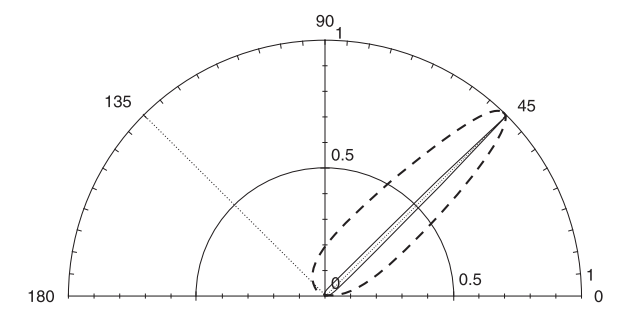
\includegraphics[scale=.6, keepaspectratio=true]{Figures/Chapter1/LWA_performance/beamwidth.PNG}}
 	\caption[Radiation patterns showing the variation of beamwidth with the change of leakage constant of a leaky-wave antenna.]{Radiation patterns for a leaky mode having $\beta/k_0=0.7071$ and two different values of $\alpha/k_0:0.1$ (dashed line) and $0.01$ (solid line) \cite{Jackson2008}.}
 	\label{fig:fixedBW}
 \end{figure}

Another interesting feature of leaky-wave antenna is that the beamwidth (between the $-3$dB points) of the main lobe varies very little with the variation of frequency. While the beam direction in Eq. \ref{eq:thetam1} depends on $\beta$, beamwidth is controlled by the attenuation constant $\alpha$. The beamwidth for uniform leaky-wave antenna is given by the following equation \cite{Jackson2008}:
%
\begin{equation}\label{eq:deltheta}
  \Delta \theta  \approx \dfrac{1}{{\dfrac{L}{{{\lambda _0}}}\cos {\theta _m}}}  \propto \dfrac{\dfrac{\alpha}{k_0}}{\cos {\theta _m}}
\end{equation}
%
where $\Delta \theta$ is the beamwidth, $\theta _m$ direction of maximum radiation and $L$ is the length of the aperture of the leaky-wave antenna. It is to be noted that the angle of radiation $\theta_m$ is dependent on frequency as shown in Eq. \ref{eq:thetam1}. However, the beamwidth $\Delta \theta$ depends on the length of the aperture $L$ in terms of wavelength $\lambda_0$. A large value of $\alpha$ indicates a short effective aperture, leading to a large beamwidth of the radiated wave. On the other hand, smaller value of $\alpha$ leads to a longer effective aperture of the antenna structure, making the beam narrower. Radiation patterns in the scanning plane for two values of $\alpha/k_0$ are presented in Fig. \ref{fig:fixedBW} \cite{Jackson2008} where radiation is achieved at an angle $\theta _m = 45^o$. In accordance with Eq. \ref{eq:deltheta}, the pattern having larger $\alpha$ value has a much larger beamwidth. Note that the radiation patterns in Fig. \ref{fig:fixedBW} do not have side-lobes because they correspond to an infinite uniform leaky-wave antenna.

Equations \ref{eq:thetam1} and \ref{eq:deltheta} suggests that as frequency is increased in a leaky-wave antenna, the main beam steers from broadside towards endfire while maintaining a constant beamwidth.

 
% \begin{figure}[!htp]
 %	\centering
% 	\noindent
 %	\subfloat[Linear Phase  \label{fig1:leaky-wave antenna}]{\includegraphics[trim={0cm 0cm 0cm 0cm},clip,scale=.6, %keepaspectratio=true]{Figures/Chapter1/leaky-wave antenna.pdf}}
 %	\caption{Leaky-wave antenna.}
% 	\label{fig:leaky-wave antenna}
 %\end{figure}


%%%%%%%%%%%%%%%%%%%%%%%%%%%%%%%%%%%%%%%%%%%%%%%%%%%%%%%%%%%%%%%%%%%%%%%%%%%%%%%%%%%%%%%%%%%%%%%%%%%%%%%%%%%%%%%%%%%%%
\section{Slot-line leaky-wave antenna} \label{sec:slotLW}

\subsection{Principle of radiation} \label{SLLWA}
 
\begin{figure} [t]
\centering
\noindent
\hspace*{\fill}%
	\mbox{\subfloat[]{
  \begin{overpic}[scale=0.35]{Figures/Chapter1/complementary/a}
				\put(10,22){\footnotesize Air }
				\put(15,46){\footnotesize I }

	\end{overpic}}}
	%
\hspace*{\fill}%
%
	\mbox{\subfloat[]{
  \begin{overpic}[scale=0.35]{Figures/Chapter1/complementary/b}
  
        \put(24.5,46){\footnotesize V }

	\end{overpic}}}
  \hspace*{\fill}%  
\caption[Complementary electric dipole in free-space and slot-line on an infinite conductive plane.]{Complementary electric dipole in free-space excited with a current $I$ (a) and slot-line on an infinite conductive plane excited with a current $V$ (b).}
\label{fig:complementary}
\end{figure} 

A slot-line on an infinite conductive plane and an electric dipole in free-space are complementary structures \cite{Kong1990}. Illustrated in Fig. \ref{fig:complementary}, antenna A is the complementary structure of antenna B. The shaded region in Fig. \ref{fig:complementary}b is an infinite ground plane. The field radiation from an electric dipole is calculated using electric currents since it radiates using electric currents. In contrast, field calculation for a slot antennas can also be done by considering nearby surface currents. However, evaluation of slot radiation becomes simpler if the source of radiation is considered to be a fictitious magnetic current. %The analysis is done by replacing the loop current by small magnetic dipoles, similar to electric dipoles. 
%
Using full-wave analytic techniques, existence of leaky-wave mode on a transversely excited slot-line was first reported in 1988 \cite{Shigesawa1988}. Following a similar approach, Neto and Maci analyzed the magnetic currents of an infinitely long slot-line placed between two homogeneous media in 2003 \cite{Neto2003}\cite{Maci2004}. The fictitious magnetic current corresponding to the slot aperture was analyzed in order to obtain and solve the dispersion relation of the slot mode. 
%
\begin{figure} [t]
\centering
\noindent
\begin{overpic}[scale=0.5]{Figures/Chapter2/fig_singleslot/singleslot}
		\put(42,38){\footnotesize Ground plane}
		\put(38,25){\footnotesize Dielectric }
		\put(35,20){\footnotesize half-space $(\epsilon_{r1})$}
		\put(33,80){\footnotesize Dielectric }
		\put(30,75){\footnotesize half-space $(\epsilon_{r2})$}
		\put(50,68){\footnotesize $z$}
		\put(90,47){\footnotesize $x$}
		\put(34,55){\footnotesize $y$}

\end{overpic}
\caption[Infinitely stretched slot located at the interface of two dielectric half spaces.]{Infinitely stretched slot located at the interface of two dielectric half spaces. The slot is etched on a ground plane \cite{Neto2003} \textcopyright 2003 IEEE.}
\label{fig:singleslot} 
\end{figure}
%
The electric dipole source excitation was expanded in the spectral domain, followed by solving the dispersion equation of the slot-line using Fourier transform. The detailed analytical expressions are beyond the scope of this thesis. In order to explain the steps in brief, an infinite slot etched in a perfect electric conductor (PEC) ground plane is illustrated in Fig. \ref{fig:singleslot}. The slot is excited by a transverse current element in $y$ direction. The upper half $(z>0)$ and lower half $(z<0)$ of the slot consist of homogeneous dielectrics while with a relative dielectric permittivity $\epsilon_{r1}$ and $\epsilon_{r2}$, respectively. The normalized magnetic current (voltage) along the slot in spectral domain is expressed as \cite{Neto2003}:

\begin{equation} \label{magcurspec}
V(k_x) = - \dfrac{2\pi}{\int_{-\infty}^{\infty} G(k_x, k_y) J_0 ( \dfrac{1}{2} w_s k_y ) d k_y} 
\end{equation}
where, $J_0$ is the Bessel function of zero order, $w_s$ is the thickness of the slot, $G(k_x, k_y)$ is the Fourier transform of Green's function of a slot placed in between two dielectric half spaces is given by 
\begin{equation} \label{slotgreen}
 G(k_x, k_y) = - \dfrac{1}{k_0 \zeta_0} \sum_{i=1}^{2} \dfrac{k_i^2 - k_x^2}{\sqrt{k_i^2 - k_x^2 - k_y^2}}
\end{equation}
where $k_0$ is the free-space propagation constant, $\zeta_0$ is the characteristic impedance, and $k_i$ for $i=1,2$ are the wave numbers in medium 1 and 2 respectively. By applying the Green's function from Eq. \ref{slotgreen} in Eq. \ref{magcurspec}, the normalized voltage along the slot-line can be obtained by applying inverse-Fourier transformation:
\begin{equation} \label{magcur}
    v(x) = \dfrac{1}{2 \pi} \int_{-\infty}^{\infty}  e^{-j k_x x} V(k_x) d k_x
\end{equation}
%
\begin{figure} [t]
\centering
\noindent
\begin{overpic}[scale=0.4]{Figures/Chapter2/fig_singleslot/lswave}
%\put(55,83){\footnotesize $\theta$ }
%\put(15,60){\footnotesize $\epsilon_{r2}$ }
%\put(15,30){\footnotesize $\epsilon_{r1}$ }
\end{overpic}
%


\caption[A radiation pattern comparing the leaky-wave and source wave radiation originating from a slot-line.]{(color inline) A sketch of a radiation pattern showing that the slot-emitted leaky wave (blue) radiates predominantly into the denser (upper) dielectric half-space. Two beams are generated since the slot-line is excited in the center. The spherical source wave (red) is competitively weaker in power.}
\label{fig:lswave} 
\end{figure}

The complex propagation constant of the leaky wave mode along the slot can be obtained by solving Eq. \ref{magcur} \cite{Neto2005}. If the upper dielectric half-space has higher dielectric permittivity than the one at the bottom ($\epsilon_{r2} > \epsilon_{r1}$), the complex propagation constant $k_x^{\mathrm{LW}}$ is given by the following equation
%
\begin{equation} \label{eq:kslot}
	k_x^{\mathrm{LW}} \approx \beta  + \dfrac{{k_d^2}}{{2\beta \left[ {1 - j\dfrac{4}{\pi }\ln \left( {\gamma_e {k_d}\dfrac{w_s}{8}} \right)} \right]}} 
\end{equation}
%
where, ${\gamma_e=\exp(\gamma)=1.781\ldots}$ is the exponential of Euler constant, $\beta$ and $k_d$, associated with the average permittivity of media 1 and 2, is expressed as 
%
\begin{subequations}
	\begin{align}
		\beta &=   \dfrac{\sqrt{k_1^2+k_1^2}} {2} \\
		k_d & =  \dfrac{\sqrt{k_2^2-k_1^2}} {2} 
	\end{align}
\end{subequations}
%
provided that medium 2 is the denser medium. Equation \ref{eq:kslot} suggests that if the width of the slot $w_s$ is very narrow, then the propagation constant of the fast wave mode along the slot ($k_x^{\mathrm{LW}} $) simplifies to be:
%
\begin{equation} \label{eq: kslotsimple}
	k_x^{\mathrm{LW}} = \beta  =  \dfrac{\sqrt{k_1^2+k_1^2}}{2} 
\end{equation}
%
which is an established expression stating the slot-line mode has a phase constant between that of the associated medium \cite{Galejs1962}.

The propagating leaky-wave mode is fast for the upper dielectric region and slow for the lower halfspace. Therefore, the slot generates leaky-wave radiation into the upper dielectric halfspace. Radiation in the denser media is obtained from Eq. \ref{eq:thetam12}:
\begin{equation} \label{eq:thetam123}
	\theta = \arcsin \dfrac{k_x^{\mathrm{LW}}}{k_2}
\end{equation}
where $k_x^{\mathrm{LW}}$ and $k_2$ is the wave number of the leaky-wave mode and radiated wave, respectively (see Fig. \ref{fig:lswave}). Equation \ref{eq:thetam123} can be simplified by applying the relation of Eq. \ref{eq: kslotsimple} as below:
%
\begin{subequations} 
	\begin{align}
		\theta & = \arcsin \dfrac{k_x^{\mathrm{LW}}}{k_2} \\
		& = \arcsin \dfrac{\dfrac{\sqrt{k_1^2+k_1^2}}{2}}{k_2} \\
		& = \arcsin \dfrac{\sqrt {\epsilon_{r1} + \epsilon_{r2}}}{2 \epsilon_{r2}} \label{eq:slottheta}
	\end{align}
\end{subequations}
where, ${\theta}$ is measured from the broadside. The direction of radiation in Fig. \ref{fig:lswave} is independent of frequency since it is a function of the permittivity values of the associated media. This implies that the leaky-wave mode in the slot produces a beam which is directed at a fixed angle irrespective of frequency. Apart from the leaky-wave radiation, the slot generates a spherical source wave from the excitation \cite{Maci2004}. The source wave contributes to the fields in the upper dielectric half-space; however, is weak when the slot is narrow in terms of wave length. Therefore it does not affect the fixed-beam performance and wide input impedance bandwidth of the slot. The polar plot in Fig. \ref{fig:lswave}  shows the leaky-wave (blue line) and spherical source wave radiation (red line) pattern originating from a  center-fed leaky-wave antenna.


%%%%%%%%%%%%%%%%%%%%%%%%%%%%%%%%%%%%%%%%%%%%%%%%%%%%%%%%%%%%%%%%%

\subsection{Fixed-beam leaky-wave antennas}

The leaky-wave radiation emitted from a slot placed at the interface of two different dielectric media can be utilized to design a fixed-beam leaky-wave antenna. There are three major designs available in the literature that involve fixed-beam leaky-wave radiation. The design principles and radiation mechanism of these antennas are described in this section.

\subsubsection{Dielectric lens}
Neto \textit{et al.} designed and built the first fixed-beam leaky-wave antenna utilizing the slot-generated leaky-wave radiation \cite{Neto2005}. The actual structure of the antenna is presented in Fig. \ref{fig:elliptical}. The design consisted of a dielectric half circle placed on top of a slot-line printed on a ground plane. The dielectric permittivity of the free-space region below the slot is lower than that of the dielectric lens. The slot-line generates leaky-wave radiation into the elliptical lens. The outer surface of the lens couples the radiation into free-space, resulting in broadside radiation. The antenna operated with a percentage bandwidth of $43\%$ ($-13$ dB $S_{11}$) and was later improved to $160\%$ ($-8.5$ dB $S_{11}$) \cite{Bruni2007} and $173\%$ \cite{Neto2010_2}. However, the overall antenna structure was electrically large. 

\begin{figure} [t!]
\centering
\noindent
\hspace*{\fill}%
	\mbox{\subfloat[]{
\begin{overpic}[scale=0.79]{Figures/Chapter1/elliptical/neto_reallens}
\end{overpic}}}
%
\hspace*{\fill}%
%
\mbox{\subfloat[]{
\begin{overpic}[trim={0cm 0cm 0cm 1.0cm},clip, scale=0.6]{Figures/Chapter1/elliptical/elliptical}
\put(10,23){\footnotesize $\epsilon_r>1$ }
\end{overpic}
\hspace*{\fill}}}%

\caption[The prototype of Neto's fixed-beam leaky-wave lens antenna and a diagram demonstrating its radiation towards broadside.]{The prototype of Neto's fixed-beam leaky-wave lens antenna \cite{Neto2010_2} \textcopyright 2010 IEEE. The dielectric lens is the white hemispherical medium (a). Cross-section of the elliptical dielectric hemisphere placed of top of a leaky-slot. The gray region illustrates the dielectric lens with a permittivity $\epsilon>\epsilon_0$. The slot is represented by the gap between ground plane at the bottom of the lens (b).}
\label{fig:elliptical} 
\end{figure}

\subsubsection{Active non-Foster circuits}
The previous design involved a dielectric lens with permittivity $\epsilon>\epsilon_0$ that coupled leaky-wave radiation into free-space. As an alternative, coupling into free-space can be achieved if the slot is located on top of a substrate with a permittivity $0<\epsilon<\epsilon_0$. In that case, air would be denser as compared to the lower permittivity dielectric substrate. Therefore, the leaky-wave radiation would directly radiate into free-space from the slot. The substrate with relative permittivity ($\epsilon_r$) below unity can be implemented through metamaterials. Metamaterials are artificially produced materials that exhibits unusual properties not found in nature. Metamaterials offer a broad range of flexibility on engineering a medium that requires exotic values of constitutive parameters ($\epsilon$ and $\mu$). However, their resonant nature limits bandwidth of operation of the antenna \cite{Enoch2002}\cite{Garcia2002}. In contrast, active structures, achievable through non-Foster circuit elements, can be used for broadband applications. Sievenpiper proposed a structure for a microstrip line using such motivation and achieved fixed-beam leaky-wave radiation over a broad bandwidth \cite{Sievenpiper2011}. The design is presented in Fig. \ref{fig:nonfoster}. Although the structure was electrically long ($10\lambda_0$), it had comparatively small thickness ($.05\lambda_0$ at the highest operating frequency). The structure operated with a percentage bandwidth of $163.64\%$. Similar fixed-beam leaky-wave antennas with a substrate having a permittivity below $1$ has been studied in \cite{Mirzaei2015} and \cite{Long2014}.
%
\begin{figure} [t!]
\centering
\noindent
\begin{overpic}[scale=0.4]{Figures/Chapter1/elliptical/nonfoster}
\put(7,13){\footnotesize \rotatebox{-18}{$0<\epsilon_r<1$}}
\put(71,70){\footnotesize Microstrip line}
\end{overpic}
\caption{Diagram of a microstrip line with a superluminal substrate that is capable to radiate leaky-wave radiation into free-space.}
\label{fig:nonfoster} 
\end{figure}

\subsubsection{Metamaterial transition layer}
In 2014, Markley \textit{et al.} utilized transformation electromagnetics to propose a design of fixed-beam leaky-wave antenna \cite{Markley2014}. The antenna radiated using slot-line leaky-wave mode and consisted of a rectangular superstrate to couple the slot-generated radiation into free-space. 

\begin{figure} [t]
\centering
\noindent
\hspace*{\fill}%
	\mbox{\subfloat[]{
  \begin{overpic}[scale=0.35]{Figures/Chapter2/fig_metaprism/metaprism_a}
				\put(10,22){\footnotesize $\theta$ }

	\end{overpic}}}
	%
\hspace*{\fill}%
%
	\mbox{\subfloat[]{
  \begin{overpic}[scale=0.35]{Figures/Chapter2/fig_metaprism/metaprism_b}
  
        \put(30,65){\footnotesize $\theta_{rad}$ }

	\end{overpic}}}
  \hspace*{\fill}%  
\caption[Illustrations of slot-line leaky-wave antenna consisting of uniform dielectric prism and anisotropic inhomogeneous metamaterial tranistion layers.]{A slot-line leaky-wave antenna with a uniform dielectric prism layer (a) and an anisotropic inhomogeneous metamaterial layer (b).}
\label{fig:metaprism}
\end{figure}

The design principle is demonstrated in Fig. \ref{fig:metaprism}. A uniform dielectric prism in Fig. \ref{fig:metaprism} coupled the radiation into free-space. Using transformation electromagnetics, the prism was transformed into a rectangular transition layer as shown in Fig. \ref{fig:metaprism}. Figure \ref{fig:loic} shows full wave simulation of an anisotropic metamaterial transition layer designed using transformation electromagnetics which is placed on top of a slot. The superstrate couples the leaky-wave mode into free-space at a desired direction. 

The design technique offered flexibility in achieving a suitable radiation angle from the antenna. However, it lead to very high values of dielectric permittivity inside the superstrate. The transition layer presented in Fig. \ref{fig:loic} resembles a matched medium with equal permittivity and permeability values. The magnetic response of the anisotropic can be implemented using resonant metamaterials, which leads to narrow bandwidth of the antenna. %\textcolor{red}{An alternative design technique proposed alongwith incorporated anisotropic metamaterials which suffers from narrowband performance.}
\begin{figure} [t!]
\centering
\noindent
\begin{overpic}[scale=0.55]{Figures/Chapter2/fig_metaprism/loic.png}

\end{overpic}
\caption[Full-wave 2D simulations of the leaky-wave mode radiating into a metamaterial slab designed to couple to free-space.]{(color inline) Full-wave 2D simulations of the traveling-wave mode radiating into a metamaterial slab designed to couple to free-space \cite{Markley2014} \textcopyright 2014 IEEE.}
\label{fig:loic} 
\end{figure}


%%%%%%%%%%%%%%%%%%%%%%%%%%%%%%%%%%%

%The purpose of the rectangular superstrate in the target domain is to imitate the hemispherical medium in the source domain and produce identical radiation pattern into free-space.
% The principal component of the leaky-wave antenna, the inhomogeneous rectangular superstrate, is designed using transformation electromagnetics to serve as a transition layer that couples the leaky-wave radiation into free-space. It is optically transformed to behave like a hemispherical uniform dielectric medium.


%%%%%%%%%%%%%%%%%%%%%%%%%%%%%%%%%%%%%%%%%%%%%%%%%%%%%%%%%%%%%%%%%%%%%%%%%%%%%%%
\section{Transformation electromagnetics} \label{sec:TO}

Transformation electromagnetics is a method of manipulating electromagnetic fields through coordinate transformation. Although the idea behind transformation optics can be dated back to 1920s \cite{gordon1923}\cite{dyson1920}, it was not until 2006 when it received great attention \cite{Pendry2006}\cite{Leonhardt2009}. Transformation optics has been widely used as a convenient tool to design novel devices such as cloaks, super lenses \cite{Pendry2000} and antennas \cite{Leonhardt2008, Lier2011, Luo2009, Popa2009, Schmiele2010, Tichit2009}.

\subsection{Form invariance property of Maxwell's equations}
The transformation electromagnetics procedure is rooted in the form invariance of Maxwell's equations. The property allows them to stay in the same form under coordinate transformations. Ward and Pendry studied the propagation of electromagnetic waves in a complex structure defined by coordinate transformation \cite{Ward1996}. The frequency domain source free Maxwell's equations are presented in equations \ref{eq:subeq1}$-$\ref{eq:subeq4} which describes how electric and magnetic fields behaves in a linear isotropic dielectric media. 

Consider a coordinate transformation from the coordinate system ${(x,y,z)}$ to ${(x', y', z')}$. The transformed medium parameters are related by a Jacobian matrix which defines the coordinate transformation. It can shown that  equations \ref{eq:subeq1}$-$\ref{eq:subeq4} stay in the same form even if they are transferred from one set of coordinate system into another \cite{ozgun2010}. The transformed space would then be characterised by material parameters $\epsilon'$ and $\mu'$, electric field $\textbf{E}'$, magnetic field $\textbf{B}'$. Maxwells' equations in the transformed space can be expressed in the following form:
%
\begin{subequations}
	\begin{align}
		\mathbf{\nabla} \cdot \mathbf{B'}    = 0 \label{eq:subeq11}\\ 
		\mathbf{\nabla} \cdot \mathbf{D'}    = 0 \label{eq:subeq12}\\
		\mathbf{\nabla} \times \mathbf{E'} + j \omega \mu \mathbf{H'} = 0 \label{eq:subeq13}\\
		\mathbf{\nabla} \times \mathbf{H'} - j \omega \epsilon \mathbf{E'} = 0 \label{eq:subeq14}
	\end{align} 
\end{subequations}
%
Generally, the  material parameters ($\epsilon'$ and $\mu'$)  in the transformed medium coordinate system turn out as tensors, typically leading to non-isotropic and inhomogeneous medium. %These inherent properties enables light to bend inside the medium, creating exotic effects. 
%%%%%%%%%%%%%%%%%%%%%%%%%%%%%%%%%%%%%%%%%%%%%%%%%%%%%%%%%%%%%
\subsection{Conformal mappings in transformation optics}
\subsubsection{Coordinate mapping}
Conformal transformation maps a coordinate system into another without varying the local angles of the coordinate grid intersections. Consider the region $\mathrm{w}$ in Fig. \ref{fig:coordinatemapping}a defined by the coordinate system $(x$,$y)$ to be mapped into the region $\mathrm{t}$ in Fig. \ref{fig:coordinatemapping}b described by the coordinate system  $(u$,$v)$. The relation between the coordinate systems of the two regions is then given by 
\begin{equation} \label{eq:transformationrelation}
	(x,y) \overset{\mathrm{f}}{\longrightarrow} (u,v) 
\end{equation}


\begin{figure} [t]
	\centering
	\noindent
	\hspace*{\fill}%    
	\subfloat[Region $\mathrm{w}$ \label{subfig1:domain1}]{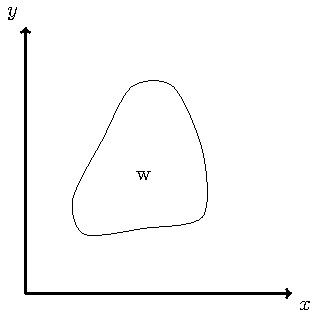
\includegraphics[trim={0cm 0cm 0cm 0cm},clip,scale=.9, keepaspectratio=true]{Figures/Chapter2/1a}}
	\hspace*{\fill}%
	\qquad
	\subfloat[Region $\mathrm{t}$   \label{subfig2:domain2}]{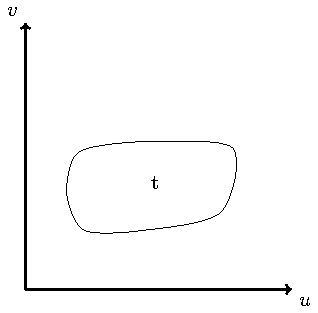
\includegraphics[trim={0cm 0cm 0cm 0cm},clip,scale=.9, keepaspectratio=true]{Figures/Chapter2/1b}}
	\hspace*{\fill}%  
	\caption[Coordinate mapping of region $\mathrm{w} = f(x,y)$ into a region $t = f(u,v)$.]{Coordinate mapping of region $\mathrm{w}$ in the $xy$ plane into a region $\mathrm{t}$ in $uv$ plane.}
	\label{fig:coordinatemapping}
\end{figure}

If $\mathrm{w}(x$,$y)$ is analytic (complex differentiable at every point) everywhere inside the domain, then $u$ and $v$ must satisfy the Cauchy-Reinmann conditions in equations \ref{eq:CR}a and \ref{eq:CR}b \cite{Saks1952}, for the mapping ($\mathrm{f}$) to be a conformal.
\begin{subequations} \label{eq:CR}
	%
	
	\begin{align}
		\dfrac{\partial u}{\partial x} &= \dfrac{\partial v}{\partial y}\\
		\dfrac{\partial u}{\partial y} &= -\dfrac{\partial v}{\partial x}
	\end{align} 
	%
\end{subequations}

Applying partial differentiation to the equations above with respect to $x$ and $y$ and relating the resulting equation, following relationships are obtained:
\begin{subequations} \label{eq:laplace}
	\begin{equation}
		\dfrac{\partial^2 u}{\partial x^2} + \dfrac{\partial^2 u}{\partial y^2} = 0
	\end{equation} 
	\begin{equation}
		\dfrac{\partial^2 v}{\partial x^2} + \dfrac{\partial^2 v}{\partial y^2} = 0
	\end{equation} 
\end{subequations}
Equations \ref{eq:laplace}a and \ref{eq:laplace}b are equivalent to Laplace's equations for analytic functions of $x(u,v)$ and $y(u,v)$. %This short derivation proves that all analytic function satisfies Laplace's equation.
%
%%%%%%%%%%%%%%%%%%%%%%%%%%%%%%%%%%%%%%%%%%%%%%%%%%%%%%%%%%%%%%%%%
\subsubsection{Local orthogonality}
It can be shown that if a conformal mapping is executed by satisfying Laplace's equation, the intersection angles of the $u$ and $v$ curves in region $\mathrm{t}$ would be the same as that of $x$ and $y$ curves in region $\mathrm{w}$ \cite{nehari1952}. In other words, conformal transformation preserves the local angles and aspect ratio between the intersecting grids. To demonstrate the local orthogonality, consider region $\mathrm{w}$ as the simplest orthogonal coordinate system: the Cartesian system, as demonstrated in Fig. \ref{fig:conformal}. 

\begin{figure}[t]
	
	\begin{center}
		
		\begin{overpic}[scale=.8]{Figures/Chapter2/conformal}
			\put(67,27){\footnotesize $\overrightarrow{dv}$}
			\put(75,20){\footnotesize $\overrightarrow{du}$}
			\put(12,15){\footnotesize $\overrightarrow{dx}$}
			\put(4,25){\footnotesize $\overrightarrow{dy}$}
			\put(10,-5){\footnotesize region $w(x,y)$}
			\put(70,-5){\footnotesize region $t(u,v)$}
		\end{overpic}
	\end{center} 
	
	\caption[Coordinate grid lines of constant $x$ and $y$ when conformally mapped from region $\mathrm{w}$ to region $\mathrm{t}$.]{Demonstration of conformal transformation. Coordinate grid lines of constant $x$ and $y$ is shown in domains $\mathrm{w}(x$,$y)$ and $\mathrm{t}(u$,$v)$.}
	\label{fig:conformal}
\end{figure}

As demonstrated in Fig. \ref{fig:conformal}, the coordinate lines of the region $\mathrm{w}(x$,$y)$ form a rectangular grid, intersecting orthogonally. There would always be a set of $u(x,y)$ and $v(x,y)$ curves that is constant for certain values of $x$ and $y$. Since $u(x,y)$ is constant in region $\mathrm{t}$, the differential $du$ would be zero. 
\begin{subequations} \label{eq:uconst}
	%
	\begin{equation}
		du = 0 
	\end{equation}  
	from the chain rule, 
	\begin{equation}
		\dfrac{\partial u}{\partial x} dx + \dfrac{\partial u}{\partial y} dy = 0 
	\end{equation}
	or,
	\begin{equation}
		\dfrac{\partial u}{\partial x} dx = - \dfrac{\partial u}{\partial y} dy 
	\end{equation}
	therefore,
	\begin{equation}
		\dfrac{dy}{dx}|_{u=\mathrm{constant}} = - \dfrac{\dfrac{\partial u}{\partial x}}{\dfrac{\partial u}{\partial y}}
	\end{equation}
	%
\end{subequations}
%
A similar relationship can be obtained for the constant $v(x,y)$ curves in region $\mathrm{t}(u$,$v)$:
\begin{equation} \label{eq:vconst}
	\dfrac{dy}{dx}|_{v=\mathrm{constant}} = - \dfrac{\dfrac{\partial v}{\partial x}}{\dfrac{\partial v}{\partial y}}
\end{equation}
Taking the product of equations \ref{eq:uconst}d and \ref{eq:vconst} and applying the Cauchy-Reinmann condition in Eq. \ref{eq:CR}:
%
\begin{equation} \label{eq:cauchy}
	\dfrac{\dfrac{\partial u}{\partial x}}{\dfrac{\partial u}{\partial y}}\dfrac{\dfrac{\partial v}{\partial x}}{\dfrac{\partial v}{\partial y}} = - \dfrac{\dfrac{\partial u}{\partial x}}{\dfrac{\partial u}{\partial y}}\dfrac{\dfrac{\partial u}{\partial y}}{\dfrac{\partial u}{\partial x}} = -1
\end{equation}
The product of the two tangents of the slope is $-1$.  Which means that the two curves $x(u,v)$ and $y(u,v)$ corresponding to constant values of $u$ and $v$ orthogonally intersect. Therefore it can be concluded that under conformal coordinate transformation, the transformed coordinate system (region $\mathrm{t}(u$,$v)$ for this case) remains locally orthogonal. The angle between the two coordinate curves are preserved at any given point if the mapping satisfies the Cauchy-Riemann condition and the plane contains constant $u$ and $v$ values corresponding to $x$ and $y$.
%
%%%%%%%%%%%%%%%%%%%%%%%%%%%%%%%%%%%%%%%%%%%%%%%%%%%%%%%%%%%%%%%%%
\subsubsection{Material parameters}

Conformal mapping can be performed by satisfying Laplace's equation between two domains provided that either of them is a rectangle. In fact, conformal map between any two domains can be found by mapping each other through a rectangle. Laplace's equation which can be solved, either analytically or numerically, to describe the transformed domain $\mathrm{t}(u$,$v)$ in Fig. \ref{fig:coordinatemapping}b. The Jacobian matrix is used to obtain its constituent material parameters ($\epsilon(u,v)$ and $\mu(u,v)$) from the solution. The Jacobian matrix of the coordinate transformation is defined as
\begin{equation} \label{jacobian}
	%
	\Lambda = \begin{bmatrix}
		\dfrac{\partial u}{\partial x} & \dfrac{\partial u}{\partial y} & 0 \\
		\dfrac{\partial v}{\partial x} & \dfrac{\partial v}{\partial y} & 0 \\
		0                             & 0                             & 1   
	\end{bmatrix}
	%
\end{equation} 
Jacobian matrix is used in coordinate transformation to transform a vector or function from one coordinate system to another. A vector function in two different coordinate system is related though the Jacobian matrix as follows:
%
\begin{subequations} \label{eq:functran}
	\begin{align}
		\mathbf{E(u,v)} & = ([\Lambda]^T)^{-1} \mathbf{E(x,y)} \\
		\mathbf{E(x,y)}  &= [\Lambda]^T \mathbf{E(u,v)}
	\end{align}
\end{subequations}
%
where $[\Lambda]^T$ is the transpose of the Jacobian matrix $\Lambda$, $\mathbf{E(x,y)}$ and $\mathbf{E(u,v)}$ are representations of o vector functions in regions $\mathrm{w}(x$,$y)$ and $\mathrm{t}(u$,$v)$, respectively. In addition, an operation, such as derivative, integral, convolution, Fourier transform, etc., can also be transformed into a new coordinate system using Jacobian matrix. Transformation of an operation $F()$ between two coordinates can be performed through the following identity: 
%
\begin{subequations} \label{eq:opctran}
	\begin{align}
		[F(u,v)] &= \dfrac{[\Lambda][F(x,y)][\Lambda]^T}{det[\Lambda]} \\
		[F(x,y)] &= det[\Lambda] [\Lambda]^{-1} [F(u,v)] ([\Lambda]^T)^{-1} 
	\end{align}
\end{subequations}
%
Using the expressions in equations \ref{eq:functran} and \ref{eq:opctran}, it can be shown that the relative permittivity $\epsilon_r(u,v)$ and relative permeability $\mu_r(u,v)$ of a conformally transformed media $\mathrm{t}(u$,$v)$ is defined through Jacobian matrix \cite{Pendry2006}.
\begin{subequations}
	\begin{align}
		[\epsilon_r(u,v)] &= \epsilon_r(x,y) \dfrac{\Lambda \Lambda^{T}}{|\Lambda|}\\
		[\mu_r(u,v)] & = \mu_r(x,y) \dfrac{\Lambda \Lambda^{T}}{|\Lambda|}
	\end{align}
\end{subequations}
where $\epsilon_r(x,y)$ and $\mu_r(x,y)$ is the relative permittivity and permeability of region $\mathrm{w}(x$,$y)$, respectively, and $|\Lambda|$ is the determinant of Jacobian matrix. $\Lambda \Lambda^{T}$ is expressed as:
\begin{equation} \label{materialjacob}
\Lambda \Lambda^{T} = \begin{bmatrix}
		\left(\dfrac{\partial u}{\partial x}\right)^2 + \left(\dfrac{\partial u}{\partial y} \right)^2 & \dfrac{\partial u}{\partial x}\dfrac{\partial v}{\partial x} +\dfrac{\partial u}{\partial y}\dfrac{\partial v}{\partial y} & 0 \\
		\dfrac{\partial u}{\partial x}\dfrac{\partial v}{\partial x} +\dfrac{\partial u}{\partial y}\dfrac{\partial v}{\partial y} & \left(\dfrac{\partial v}{\partial x}\right)^2 + \left(\dfrac{\partial v}{\partial y} \right)^2 & 0 \\
		0                             & 0                             & 1   
	\end{bmatrix}
	%
\end{equation} 
It should be noted that this two-dimensional transformation is applicable only for transversely (in the direction out of the page) polarized electric or magnetic fields. If Cauchy-Reinmann conditions in Eq. \ref{eq:CR} are used in Eq. \ref{materialjacob}, the matrices can be simplified into the following equations to find the material parameters in region $\mathbf{t(u,v)}$
\begin{subequations}\label{matpar}	
	\begin{align} 
		[\epsilon_r(u,v)] = \epsilon_r(x,y)
		\begin{bmatrix}
			1 & 0 & 0 \\
			0 & 1 & 0 \\
			0 & 0 & \dfrac{1}{|\Lambda|}   
		\end{bmatrix} \\
		[\mu_r(u,v)] =  \mu_r(x,y)
		\begin{bmatrix}
			1 & 0 & 0 \\
			0 & 1 & 0 \\
			0 & 0 & \dfrac{1}{|\Lambda|}   
		\end{bmatrix}
	\end{align}	
\end{subequations}
%
Equations \ref{matpar} describe an isotropic, inhomogeneous and matched medium, an inherent property of conformal transformation \cite{Leonhardt2009}. Conformal method has been utilized to study optical cloaks \cite{Urzhumov2010}, carpet cloaks \cite{Schmied2010}, antennas \cite{Leonhardt2008}, waveguides \cite{Ma2010}. Inhomogeneous media can be defined by space-dependent index of refraction and are referred to as graded index media \cite{Gomez-Reino1987}. Gradient index are non resonant and are therefore prefered over resonant metamaterials for broadband implementations.
%However, dielectric materials with a permeability greater than unity is difficult to obtain. Therefore, practically applications employ quasi-conformal transformation, a subset of conformal transformation optics, that gives rise to isotropic inhomogeneous media with unity permeability.

%General transformation optics method results in anisotropic inhomogeneous media which is employed by exotic materials known as metamaterials \cite{Eleftheriades2002}. However, metamaterials resonate within a very narrow bandwidth, which can be a limitation for many broadband applications. For this reason, most anisotropic media designed through transformation optics are physically realized by choosing a particular polarization for the ingoing light. 

The material constituent parameters of a conformally transformed medium is isotropic with equal permittivity and permeability, (see Eq. \ref{matpar}). However, designing a medium with wide-range of permeability values is difficult in practice. Unity permeability value in the transformed medium can be achieved for a the right polarization of wave. Equation \ref{matpar} suggests that both permittivity and permeability tensors of the transformed medium contain $z$ components ($\epsilon_{33}$ and $\mu_{33}$) in the diagonal entries. For a $z$ polarized wave only $\epsilon_{33}$ from Eq.\ref{matpar}a and and $\mu_{33}$ from Eq.\ref{matpar}b affects the electromagnetic behaviour of the transformed medium \cite{zouhdi2012}\cite{Leonhardt2009}. Therefore, Eqs. Eq.\ref{matpar}a and Eq.\ref{matpar}b can be simplified as follows:
%
\begin{subequations} \label{eq:eps}
	\begin{align}
		\epsilon_r(u,v) &=\dfrac{\epsilon_r(x,y)}{|\Lambda|} \\
                         &=\dfrac{\epsilon_r(x,y)}{\sqrt{\left(  \dfrac{du}{dx}\right )^{2}+\left(\dfrac{du}{dy}\right )^{2}}} \\
		&=\dfrac{\epsilon_r(x,y)}{\sqrt{\dfrac{du}{dx}\dfrac{dv}{dy}-\dfrac{du}{dy}\dfrac{dv}{dx}}} \\
		&=\dfrac{\epsilon_r(x,y)}{\sqrt{\left(\dfrac{dv}{dx}\right )^{2}+\left(\dfrac{dv}{dy}\right )^{2}}} \label{eq:transconda}
	\end{align}
\end{subequations}
%
and
%
\begin{equation} \label{eq:transcondb}
	\mu_r(u,v) = 1
\end{equation}
%

%%%%%%%%%%%%%%%%%%%%%%%%%%%%%%%%%%%%%%%%%%%%%%%%%%%%%%%%%%%%%%%%%%%%%
\subsection{Inverse transformation}

\begin{figure}[t]
	
	\begin{center}
		
		\begin{overpic}[scale=.5]{Figures/Chapter1/inverse_transformation/inverse}
			\put(10,-5){\footnotesize Region $\mathrm{w}(x$,$y)$}
			\put(66,-5){\footnotesize Target region $\mathrm{t}(u$,$v)$}
			\put(39,50){\footnotesize Transformation}
			\put(48,46){\footnotesize ($f$)}
			\put(30,37){\footnotesize $\epsilon_r(x,y)$, $\mu_r(x,y)$}
			\put(34,8){\footnotesize Inverse transformation}
			\put(47,4){\footnotesize ($f^{-1}$)}
			\put(86,37){\footnotesize $\epsilon_r(u,v)$, $\mu_r(u,v)$}
		\end{overpic}
	\end{center} 
	
	\caption{Transformation and inverse transformation between region $\mathbf{w}$ and $\mathbf{t}$.}
	\label{fig:inverse}
\end{figure}

Inverse transformation follows the equations of transformation optics by mapping the inhomogeneous transformed domain back to the homogeneous initial domain \cite{Zhang2010}. That is, Laplace's equation is solved for the transformed space to define the medium in an original space. The relationship between the two regions in Fig. \ref{fig:conformal} can be described by:
\begin{equation} 
	(u,v) \overset{\mathrm{f^{-1}}}{\longrightarrow} (x,y) 
\end{equation}
%
Note that the relation is the inverse of Eq. \ref{eq:transformationrelation}. The process of inverse transformation is illustrated in Fig. \ref{fig:inverse}. The coordinate mapping relationship is represented by $f^{-1}$. Once the solution of the inverse transformation is known by solving Laplace's equation, the material parameters are modified by inverting the Jacobian expression in equations \ref{eq:transconda} and \ref{eq:transcondb} and expressed as:
\begin{subequations} \label{eq:inversetran}
	\begin{align}
		\epsilon_r(x,y) &=\epsilon_r(u,v) \sqrt{\dfrac{dv}{dx}^{2}+\dfrac{dv}{dy}^{2}}  \\
		\mu_r(x,y) &=1
	\end{align}   
\end{subequations}
Equations \ref{eq:inversetran} can be used to inversely transform a transformed media back into its original domain. The technique presented in Ch. \ref{Chapter2} of this thesis utilizes the inverse transformation method which is later used in Ch. \ref{Chapter3} to develop a fixed-beam leaky-wave antenna. 
%%%%%%%%%%%%%%%%%%%%%%%%%%%%%%%%%%%%%%%%%%%%%%%%%%%%%%%%%%%%%%%%%%%%%%%%
%\section{Summary}

%Almost all leaky-wave antennas initially designed generated radiation utilizing a propagating fast wave. It was later found out that although slow waves do not fundamentally radiate, but can be made to radiate by spatially modulating the transmission line. Based on whether it supports a fast wave or a slow wave, leaky-wave antennas can be categorized into two types: uniform leaky-wave antenna, and periodic leaky-wave antenna \cite{Jackson2008}.